\documentclass{rvcepaper}
\begin{document}

% ---------- HS351TA Entrepreneurship & IPR (CIE-II)
\begin{iempaperB}
\paperinfo{ayear={2024-2025 (ODD Sem)},date={07/01/2025},code={HS351TA},sem={V},exam={CIE -II},maxmarks={10 + 50},duration={120 Min},
 title={ENTREPRENEURSHIP AND INTELLECTUAL PROPERTY RIGHTS}}
\iemheadB
\begin{cietable}{M}{BT}{CO}
\qpart{Part -- A}
\q{1}{\blank[1.5cm] component is key in assessing market feasibility}{1}{1}{2}
\q{2}{What does break-even analysis determine?}{1}{1}{3}
\q{3}{Which strategy in Porter's generic strategies focuses on offering unique products?}{1}{1}{3}
\q{4}{What does a proof of concept primarily demonstrate?}{1}{1}{2}
\q{5}{Why is prototyping important in the ideation process?}{2}{1}{2}
\q{6}{In order to register Industrial Design, Design should be new and \blank[1.8cm]}{1}{1}{4}
\q{7}{Can a colour by itself be subject matter of registration of industrial design? If yes, justify your statement.}{2}{2}{4}
\q{8}{Upon expiry of registration of a design under Designs Act 2000 it becomes \blank[1.8cm] property}{1}{1}{4}
\qpart{Part --B}
\q{1}{A medium-sized technology company in India develops an innovative algorithm for optimizing supply chain logistics. To maintain its competitive edge, the company decides not to patent the algorithm but to treat it as a trade secret. Over time, a former employee joins a competitor and allegedly discloses key aspects of the algorithm. The company must navigate the legal landscape to protect its trade secrets.\newline
\textbf{Questions:}
\begin{rom}
\item[i.] What legal tools and mechanisms are available in India to protect trade secrets?
\item[ii.] Analyze the company's decision to treat the algorithm as a trade secret instead of patenting it. What are the advantages and risks of this approach?
\end{rom}
What preventive measures could the company have implemented to minimize the risk of trade secret leakage?}{10}{3}{4}
\q{2}{A furniture design firm creates a unique chair design that combines aesthetics with ergonomic principles. The design becomes a market hit, but a competitor begins manufacturing and selling a chair with an almost identical appearance. The firm initiates legal proceedings to obtain design protection and stop the competitor's activities.\newline
Questions:
\begin{rom}
\item[i.] What features of the chair design qualify it for industrial design protection?
\end{rom}}{10}{3}{4}
\end{cietable}
\end{iempaperB}

% ---------- IM352IA Operations Management (CIE - II)
\begin{iempaperB}
\paperinfo{ayear={2024-2025 (ODD Sem)},date={07 January 2025},code={IM352IA},sem={V},exam={CIE -- II},maxmarks={10 + 50},duration={120 Min},
 title={OPERATIONS MANAGEMENT}}
\iemheadB
\begin{cietable}{M}{BT}{CO}
\qpart{Part -- A}
\q{1}{In services, the process structure is primarily influenced by the level of \blank[1cm] and customization.}{1}{1}{2}
\q{2}{In manufacturing, a \blank[1.5cm] process is ideal for high-volume, standardized production.}{1}{2}{2}
\q{3}{The first step in a systematic approach to long-term capacity decisions is \blank[1.5cm] future demand.}{1}{2}{2}
\q{4}{A systematic approach to capacity planning involves forecasting, identifying alternatives, and evaluating \blank[1.8cm].}{1}{1}{2}
\q{5}{The \blank[1.5cm] component of a forecast captures recurring patterns over specific periods, such as seasons or months.}{1}{2}{3}
\q{6}{The smoothing constant in exponential smoothing ranges between 0 and \blank[1.8cm].}{1}{1}{3}
\q{7}{\blank[0.8cm] provides a detailed plan of what needs to be produced and when, serving as an input for MRP.}{1}{1}{3}
\q{8}{The \blank[0.8cm] file contains information about the quantities of materials required to make a product.}{1}{2}{3}
\q{9}{\blank[1.2cm] integrates all business processes, including finance, HR, and supply chain, into a unified system.}{1}{2}{3}
\q{10}{\blank[1.2cm] ensures that operational capabilities are in line with the company's strategic goals.}{1}{2}{3}
\qpart{Part --B}
\q{1}{Explain the major process strategy decisions and their implications for operations.}{10}{2}{2}
\q{2}{Richard Garber is the head designer for Matthews and Novak Design Company. Garber has been called in to design the layout for a newly constructed office building. From statistical samplings over the past three months, Garber developed the following closeness matrix for daily trips between the department's offices.\newline
\textbf{a.} If other factors are equal, which two offices should be located closest together?\newline
\textbf{b.} Figure shows an alternative layout for the department. What is the total weighted-distance score for this plan based on rectilinear distance and assuming that offices A and B are three units of distance apart?
\par\vspace{4pt}\noindent\begin{minipage}[c]{7.2cm}\centering\small
{\bfseries CLOSENESS MATRIX}\\[1pt]
\renewcommand{\arraystretch}{1.1}\setlength{\tabcolsep}{3pt}
\begin{tabular}{|c|c|c|c|c|c|c|}
\hline \multicolumn{1}{|c|}{} & \multicolumn{6}{c|}{Trips Between Departments}\\\hline
Department & A & B & C & D & E & F\\\hline
A & --- & 25 & 90 & & 105 & 185\\\hline
B & & --- & & & 125 & 125\\\hline
C & & & --- & & 25 & \\\hline
D & & & & --- & & 105\\\hline
E & & & & & --- & \\\hline
F & & & & & & ---\\\hline
\end{tabular}\end{minipage}\hspace{0.3cm}\begin{minipage}[c]{3.8cm}\centering
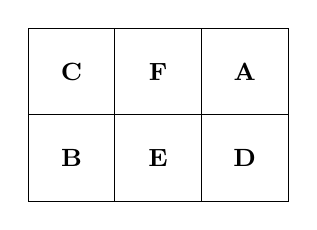
\begin{tikzpicture}[x=1.1cm,y=1.1cm]\draw (0,0) rectangle (3,2);\draw (1,0)--(1,2);\draw (2,0)--(2,2);\draw (0,1)--(3,1);
\node at (0.5,1.5) {\small\bfseries C};\node at (1.5,1.5) {\small\bfseries F};\node at (2.5,1.5) {\small\bfseries A};
\node at (0.5,0.5) {\small\bfseries B};\node at (1.5,0.5) {\small\bfseries E};\node at (2.5,0.5) {\small\bfseries D};\end{tikzpicture}\end{minipage}}{10}{3}{2}
\q{3}{The monthly demand for units manufactured by the Acme Rocket Company has been as follows:
\qtabc{|l|l|l|l|}{\hline Month & Units & Month & Units\\\hline May & 100 & September & 105\\\hline June & 80 & October & 110\\\hline July & 110 & November & 125\\\hline August & 115 & December & 120\\\hline}
\textbf{i.} Use the exponential smoothing method to forecast the number of units for June to January. The initial forecast for May was 105 units; $\alpha=0.2$.\newline
\textbf{ii.} Calculate the absolute percentage error for each month from June through December and the MAD and MAPE of forecast error as of the end of December.\newline
\textbf{iii.} Calculate the tracking signal as of the end of December. What can you say about the performance of your forecasting method?}{10}{3}{3}
\q{4}{Refer to the bill of materials for product A. If there is no existing inventory and no scheduled receipts, how many units of items G, E, and D must be purchased to produce five units of end item A?
\par\vspace{4pt}\centerline{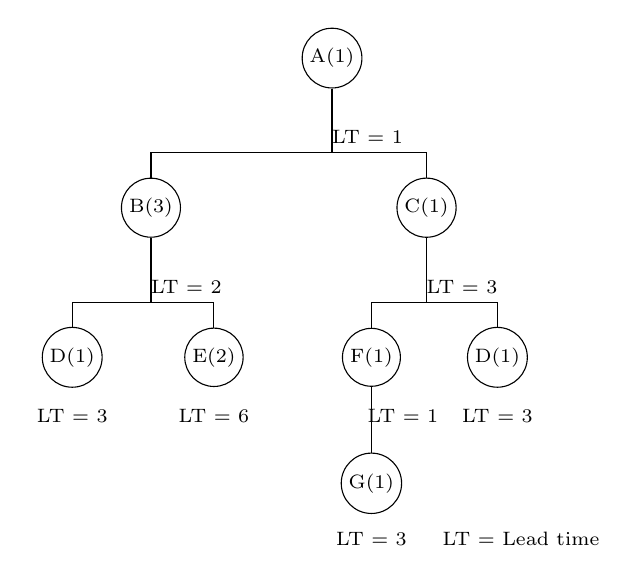
\begin{tikzpicture}[x=1cm,y=1cm,font=\scriptsize,every node/.style={},nd/.style={circle,draw,inner sep=1.5pt,minimum size=0.55cm}]
\node[nd] (A) at (0,0) {A(1)}; \node[nd] (B) at (-2.3,-1.9) {B(3)}; \node[nd] (C) at (1.2,-1.9) {C(1)};
\node[nd] (D1) at (-3.3,-3.8) {D(1)}; \node[nd] (E) at (-1.5,-3.8) {E(2)}; \node[nd] (F) at (0.5,-3.8) {F(1)}; \node[nd] (D2) at (2.1,-3.8) {D(1)};
\node[nd] (G) at (0.5,-5.4) {G(1)};
\draw (A) -- (0,-1.2) -| (B); \draw (0,-1.2) -| (C); \node at (0.45,-1.0) {LT = 1};
\draw (B) -- (-2.3,-3.1) -| (D1); \draw (-2.3,-3.1) -| (E); \node at (-1.85,-2.9) {LT = 2};
\draw (C) -- (1.2,-3.1) -| (F); \draw (1.2,-3.1) -| (D2); \node at (1.65,-2.9) {LT = 3};
\draw (F) -- (G);
\node at (-3.3,-4.55) {LT = 3}; \node at (-1.5,-4.55) {LT = 6}; \node at (0.9,-4.55) {LT = 1}; \node at (2.1,-4.55) {LT = 3}; \node at (0.5,-6.1) {LT = 3}; \node at (2.4,-6.1) {LT = Lead time};
\end{tikzpicture}}\par}{10}{4}{3}
\q{5}{Explain how the concept of dependent demand in material requirements planning is fundamental to resource planning.}{10}{2}{3}
\end{cietable}
\btfoot{|c|c|c|*{10}{C{0.85cm}|}}{\hline
\multirow{3}{*}{\bfseries Marks Distribution} & \multicolumn{2}{c|}{\bfseries Particulars} & CO1 & CO2 & CO3 & CO4 & L1 & L2 & L3 & L4 & L5 & L6\\\cline{2-13}
 & Quiz & \multirow{2}{*}{Max Marks} & -- & 4 & 6 & -- & 4 & 6 & -- & -- & -- & --\\\cline{2-2}\cline{4-13}
 & Test & & -- & 20 & 30 & -- & -- & 20 & 20 & 10 & -- & --\\\hline}
\stars{*******}
\end{iempaperB}

% ---------- IM353IA Quality Assurance (CIE - II)
\begin{iempaperB}
\paperinfo{ayear={2024-2025 (ODD Sem)},usn=0,date={7\textsuperscript{th} January 2025},code={IM353IA},sem={V},exam={CIE -- II},maxmarks={50},duration={90 Min},
 title={QUALITY ASSURANCE}}
\iemheadB
\ptitlem{PART -- A}{Max Marks: 10}
\begin{cietable}{M}{BT}{CO}
\q{1.}{Differentiate between Attribute control chart and Variable control chart.}{2}{L2}{CO1}
\q{2.}{What does an R-chart measure, and why is it important in statistical process control?}{2}{L1}{CO2}
\q{3.}{What is the key difference between a p-chart and a np-chart?}{2}{L2}{CO3}
\q{4.}{Expand the acronyms: AQL, UTPD}{2}{L2}{CO3}
\q{5.}{Write two applications of acceptance sampling.}{2}{L2}{CO2}
\end{cietable}
\ptitlem{PART -- B}{}
\begin{cietable}{M}{BT}{CO}
\q{1.}{A TiW layer is deposited on a substrate using a sputtering tool. The following table contains layer thickness measurements (in Angstroms) on 10 subgroups of four substrates. Set up $\bar{X}$ and $s$ charts on this process and compute trial control limits.
\qtabc{|c|c|c|c|c|}{\hline \textbf{Subgroup} & $\mathbf{x_1}$ & $\mathbf{x_2}$ & $\mathbf{x_3}$ & $\mathbf{x_4}$\\\hline 1 & 459 & 449 & 435 & 450\\\hline 2 & 443 & 440 & 442 & 442\\\hline 3 & 457 & 444 & 449 & 444\\\hline 4 & 469 & 463 & 453 & 438\\\hline 5 & 443 & 457 & 445 & 454\\\hline 6 & 444 & 456 & 456 & 457\\\hline 7 & 445 & 449 & 450 & 445\\\hline 8 & 446 & 455 & 449 & 452\\\hline 9 & 444 & 452 & 457 & 440\\\hline 10 & 432 & 463 & 463 & 443\\\hline}}{10}{3}{CO3}
\q{2.}{Write a note on Standardized control chart. What is the process capability? Explain any one of the techniques of process capability analysis.}{10}{2}{CO1}
\q{3.}{Lots of Bushing screws from a single supplier were inspected 100 percent with the following results.
\qtabc{|c|c|c|}{\hline Lot No. & Amount in lot & Number rejected\\\hline 1 & 6000 & 183\\\hline 2 & 6000 & 131\\\hline 3 & 10000 & 184\\\hline 4 & 1783 & 23\\\hline 5 & 3089 & 171\\\hline 6 & 5774 & 65\\\hline 7 & 3000 & 46\\\hline 8 & 2724 & 85\\\hline}
Draw an appropriate control chart for the data. What can you conclude on the state of control?}{10}{2}{CO2}
\q{4.}{Draw the OC Curve, AOQ Curve, ASN Curve and ATI Curve for the single sampling plan with N = 5000, n = 100 and c = 2}{10}{4}{CO4}
\q{5.}{A factory inspects different samples of a product, recording the number of defects in each sample. The sample size is constant, and the number of defects is provided below:
\qtabc{|c|c|}{\hline Sample No. & Number of Defects\\\hline 1 & 5\\\hline 2 & 8\\\hline 3 & 6\\\hline 4 & 4\\\hline 5 & 7\\\hline 6 & 9\\\hline 7 & 5\\\hline 8 & 6\\\hline}
\begin{romi}
\item Draw an appropriate control chart for the data. Evaluate the process.
\item Plot the centreline, upper control limit (UCL), and lower control limit (LCL).
\end{romi}}{10}{2}{CO2}
\end{cietable}
\btfoot{|c|c|c|*{8}{C{0.85cm}|}}{\hline
\multirow{3}{*}{\bfseries Marks Distribution} & \multicolumn{2}{c|}{\bfseries Particulars} & CO1 & CO2 & CO3 & CO4 & L1 & L2 & L3 & L4\\\cline{2-11}
 & Quiz & \multirow{2}{*}{Max Marks} & 02 & 04 & 04 & -- & 2 & 8 & -- & --\\\cline{2-2}\cline{4-11}
 & Test & & 10 & 20 & 10 & 10 & -- & 30 & 10 & 10\\\hline}
\stars{*******}
\end{iempaperB}

% ---------- IM254TA Financial Accounting and Costing (CIE - II)
\begin{iempaperB}
\paperinfo{ayear={2024-2025 (ODD Sem)},date={8\textsuperscript{th} January 2025},code={IM254TA},sem={V Semester},exam={CIE -- II},maxmarks={10 + 50},duration={120 Mins},
 title={FINANCIAL ACCOUNTING AND COSTING}}
\iemheadB
\ptitle{PART -- A}
\begin{cietable}{M}{BT}{CO}
\q{1}{What is a Trial Balance, and why is it prepared?}{02}{2}{CO2}
\q{2}{How is Gross Profit calculated?}{02}{1}{CO3}
\q{3}{Why is depreciation included in the Income Statement?}{02}{2}{CO3}
\q{4}{What is the basic accounting equation represented in a Balance Sheet?}{02}{1}{CO3}
\q{5}{What is the difference between current and non-current assets?}{02}{1}{CO1}
\end{cietable}
\ptitle{PART -- B}
\begin{cietable}{M}{BT}{CO}
\q{1.}{The following are the ledger balances of a business as of December 31, 2024. Prepare a trail balance.
\qtab{|l|r|l|}{\hline \multicolumn{1}{|c|}{\textbf{Account}} & \multicolumn{1}{c|}{\textbf{Amount (\rupee)}} & \textbf{Type}\\\hline Cash & 50,000 & Debit\\\hline Capital & 1,50,000 & Credit\\\hline Sales & 2,00,000 & Credit\\\hline Purchases & 1,00,000 & Debit\\\hline Furniture & 25,000 & Debit\\\hline Salaries & 30,000 & Debit\\\hline Accounts Receivable & 45,000 & Debit\\\hline Accounts Payable & 40,000 & Credit\\\hline}}{10}{3}{CO2}
\q{2.}{Prepare a Profit and Loss Account for Green Enterprises for the year ending December 31, 2024, from the following details:
\qtabc{|l|r|}{\hline \multicolumn{1}{|c|}{\textbf{Particulars}} & \multicolumn{1}{c|}{\textbf{Amount (\rupee)}}\\\hline Sales Revenue & 7,50,000\\\hline Purchases & 4,00,000\\\hline Opening Inventory & 1,20,000\\\hline Closing Inventory & 80,000\\\hline Wages & 50,000\\\hline Office Expenses & 40,000\\\hline Utilities & 30,000\\\hline Depreciation on Machinery & 20,000\\\hline}}{10}{4}{CO3}
\q{3.}{Prepare a Balance Sheet for Green Valley Enterprises as of December 31, 2024, from the following details:
\qtabc{|l|r|l|r|}{\hline \multicolumn{1}{|c|}{\textbf{Particulars}} & \multicolumn{1}{c|}{\textbf{Amount (\rupee)}} & \multicolumn{1}{c|}{\textbf{Particulars}} & \multicolumn{1}{c|}{\textbf{Amount (\rupee)}}\\\hline Capital & 5,00,000 & Cash & 1,00,000\\\hline Bank Loan & 3,00,000 & Building & 5,00,000\\\hline Accounts Payable & 1,50,000 & Inventory & 2,00,000\\\hline Salaries Payable & 50,000 & Furniture & 80,000\\\hline Accounts Receivable & 1,20,000 & Equipment & 1,50,000\\\hline}}{10}{3}{CO3}
\q{4.}{From the following information, prepare a cost sheet for XYZ Manufacturing Co. for the year ending March 31, 2025:
\qtabc{|l|r|}{\hline \multicolumn{1}{|c|}{\textbf{Particulars}} & \multicolumn{1}{c|}{\textbf{Amount (\rupee)}}\\\hline Raw Materials Consumed & 3,00,000\\\hline Direct Labor & 2,00,000\\\hline Factory Overheads & 80,000\\\hline Office and Administrative Overheads & 40,000\\\hline Selling and Distribution Overheads & 30,000\\\hline Opening Stock of Finished Goods & 50,000\\\hline Closing Stock of Finished Goods & 60,000\\\hline Profit Percentage on Cost & 25\%\\\hline}}{10}{3}{CO4}
\q{5.}{Explain the three main elements of cost sheet with examples. How are they classified and used in cost accounting?}{10}{3}{CO4}
\end{cietable}
\btfoot{|c|c|c|*{11}{C{0.82cm}|}}{\hline
\multirow{3}{*}{\bfseries Marks Distribution} & \multicolumn{2}{c|}{\bfseries Particulars} & CO1 & CO2 & CO3 & CO4 & CO5 & L1 & L2 & L3 & L4 & L5 & L6\\\cline{2-14}
 & \multirow{2}{*}{Max Marks} & Quiz & 02 & 02 & 06 & -- & -- & 06 & 04 & -- & -- & -- & --\\\cline{3-14}
 & & Test & -- & 10 & 20 & 20 & -- & -- & -- & 30 & 20 & -- & --\\\hline}
\stars{*****}
\end{iempaperB}

% ---------- IM355TBD Advanced Decision Modelling (CIE - 2)
\begin{iempaperB}
\paperinfo{ayear={2024-2025 (ODD Sem)},usn=0,date={9\textsuperscript{th} January 2025},code={IM355TBD},sem={V},exam={CIE -- 2},maxmarks={50},duration={90 Min},
 title={ADVANCED DECISION MODELLING (Professional Core Elective)}}
\iemheadB
\begin{cietable}{M}{BT}{CO}
\qpart{Part A}
\q{1.}{Mention the situations that make the replacement of items necessary?}{02}{2}{1}
\q{2.}{What are the three strategies of replacement of items which follow sudden failure mechanisms?}{02}{2}{3}
\q{3.}{State two differences between preventive maintenance and breakdown maintenance.}{02}{2}{2}
\q{4.}{Give one advantage and one disadvantage of individual replacement policies.}{02}{2}{2}
\q{5.}{State the main objectives of using the EOQ model?}{02}{1}{3}
\qpart{Part B}
\q{1}{A firm is considering the replacement of a machine, whose cost price is Rs 12,200, and its scrap value is Rs 200. From experience the running (maintenance and operating) costs are found to be as follows:
\qtabc{|l|c|c|c|c|c|c|c|c|}{\hline Year: & 1 & 2 & 3 & 4 & 5 & 6 & 7 & 8\\\hline Running Cost (Rs): & 200 & 500 & 800 & 1200 & 1800 & 2500 & 3200 & 4000\\\hline}
When should the machine be replaced?}{10}{3}{1}
\q{2}{The data on the running costs per year and resale price of equipment A, whose purchase price is Rs 2,00,000 are as follows:
\qtabc{|l|c|c|c|c|c|c|c|}{\hline Year: & 1 & 2 & 3 & 4 & 5 & 6 & 7\\\hline Running cost (Rs): & 30,000 & 38,000 & 46,000 & 58,000 & 72,000 & 90,000 & 1,10,000\\\hline Resale value (Rs): & 1,00,000 & 50,000 & 25,000 & 12,000 & 8,000 & 8,000 & 8,000\\\hline}
\begin{romi}
\item What is the optimum period of replacement?
\item When equipment A is two years old, equipment B, which is a new model for the same usage, is available. The optimum period for replacement is 4 years with an average cost of Rs 72,000. Should equipment A be changed with equipment B? If so, when?
\end{romi}}{10}{3}{2}
\q{3}{A company is considering the purchase of a new machine at Rs 15,000. The economic life of the machine is expected to be 8 years. The salvage value of the machine at the end of the life will be Rs 3,000. The annual running cost is estimated to be Rs 7,000.
\begin{romi}
\item Assuming an interest rate of 5 per cent, determine the present worth of future costs of the proposed machine.
\item Compare the new machine with the presently-owned machine that has an annual operating cost of Rs 5,000 and cost of repair Rs 1,500 in the second year, with an annual increase of Rs 500 in the subsequent years of its life.
\end{romi}}{10}{3}{3}
\q{4}{The following failure rates have been observed for a certain type of bulbs.
\qtabc{|l|c|c|c|c|c|c|c|c|}{\hline End of Week: & 1 & 2 & 3 & 4 & 5 & 6 & 7 & 8\\\hline Probability of failure to date: & 0.05 & 0.13 & 0.25 & 0.43 & 0.68 & 0.88 & 0.96 & 1.0\\\hline}
The cost of replacing an individual bulb is Rs. 2.25. if the cost of group replacement is 60 paisa per bulb and the total number of bulbs is 1000. What is best interval between group replacements?}{10}{3}{3}
\q{5}{Differentiate between Continuous Review and Periodic Review Inventory Systems by the following aspects:
\begin{romi}
\item Monitoring
\item Reorder Trigger
\item Stockouts Risks
\item System Complexity
\item Suitability
\end{romi}}{10}{2}{2}
\end{cietable}
\btfoot{|c|c|c|*{10}{C{0.85cm}|}}{\hline
\multirow{3}{*}{\bfseries Marks Distribution} & \multicolumn{2}{c|}{\bfseries Particulars} & CO1 & CO2 & CO3 & CO4 & L1 & L2 & L3 & L4 & L5 & L6\\\cline{2-13}
 & Quiz & Max Marks & 1 & 2 & 2 & -- & 1 & 2 & 2 & -- & -- & --\\\cline{2-13}
 & Test & Max Marks & 10 & 20 & 20 & -- & -- & 10 & 40 & -- & -- & --\\\hline}
\stars{*******}
\end{iempaperB}

\end{document}
